\documentclass{article}

\usepackage[utf8]{inputenc}
\usepackage[francais]{babel}
\usepackage{geometry}
\usepackage{amsfonts}

% drawing
\usepackage{pgf,tikz}
\usetikzlibrary{arrows}

\title{Pliage}
\author{\'Eloi Perdereau}
\date{\today}

\sloppy
\geometry{dvips,a4paper,margin=1in}

\begin{document}
\maketitle

\section{Définition de la scène (voir figure 1)}
Soit $e$ une arête concave, $[ab]$ le dernier segment du chemin à étendre tel que $a$ domine $b$ et $b \in e$. Soit $P_{max}$ le plan contenant $e$ et $[ab]$, et $P_{min}$ le plan plat de l'obstacle.\\
Soit $q_{min}$ et $q_{max}$ les points d'intersections des plans $P_{min}$ et $P_{max}$ respectivement. On note $\theta_{max}$ l'angle $\angle{q_{min} b q_{max}}$.
On cherche à calculer l'angle $\theta^*$ tel que si on applique à $P_{max}$ une rotation de $\theta_{max}-\theta^*$ autour de $e$ (pliage), alors l'image de la droite $(ab)$ sur ce plan intersecte $d$ en un point $q^*$ qui sera l'extension voulue du chemin. \\

\section{Calcul de $\theta^*$}
En regardant la projection sur le plan $(xy)$ ($e$ varie selon $z$ uniquement), on peut calculer $\theta_{max}$ :
\[cos(\theta_{max}) = \frac{|\vec{bq_{min}}|}{|\vec{bq_{max}}|}\]

\definecolor{qqwuqq}{rgb}{0,0.39,0}
\definecolor{zzttqq}{rgb}{0.6,0.2,0}
\definecolor{uuuuuu}{rgb}{0.27,0.27,0.27}
\definecolor{xdxdff}{rgb}{0.49,0.49,1}
\definecolor{wqwqwq}{rgb}{0.38,0.38,0.38}
\definecolor{qqqqff}{rgb}{0,0,1}
\begin{tikzpicture}[line cap=round,line join=round,>=triangle 45,x=1.0cm,y=1.0cm]
\clip(-2,-3.19) rectangle (5,8.01);
\fill[color=zzttqq,fill=zzttqq,fill opacity=0.1] (2.96,0) -- (0,0) -- (0,-2.96) -- (2.96,-2.96) -- cycle;
\draw [shift={(0,0)},color=qqwuqq,fill=qqwuqq,fill opacity=0.1] (0,0) -- (0:0.73) arc (0:65.17:0.73) -- cycle;
\draw [color=wqwqwq,domain=-2:5] plot(\x,{(-0--1.81*\x)/0.84});
\draw (2.96,-3.19) -- (2.96,8.01);
\draw [color=zzttqq] (2.96,0)-- (0,0);
\draw [color=zzttqq] (0,0)-- (0,-2.96);
\draw [color=zzttqq] (0,-2.96)-- (2.96,-2.96);
\draw [color=zzttqq] (2.96,-2.96)-- (2.96,0);
\draw [color=wqwqwq,domain=-2:5] plot(\x,{(-0-0*\x)/2.96});
\draw [color=wqwqwq](-1.64,0.52) node[anchor=north west] {$P_{min}$};
\draw [color=wqwqwq](3.64,7.57) node[anchor=north west] {$P_{max}$};
\draw (2.62,7.93) node[anchor=north west] {d};
\begin{scriptsize}
\draw [fill=qqqqff] (-0.84,-1.81) circle (1.5pt);
\draw[color=qqqqff] (-1.01,-1.54) node {$a$};
\draw [fill=qqqqff] (0,0) circle (1.5pt);
\draw[color=qqqqff] (-0.26,-0.09) node {$b$};
\draw[color=wqwqwq] (4.78,9.56) node {$P_{max}$};
\draw [fill=xdxdff] (2.96,0) circle (1.5pt);
\draw[color=xdxdff] (3.28,0.47) node {$q_{min}$};
\draw[color=black] (3.09,9.31) node {$d$};
\draw [fill=uuuuuu] (2.96,6.41) circle (1.5pt);
\draw[color=uuuuuu] (3.35,6.65) node {$q_{max}$};
\draw[color=zzttqq] (1.53,-1.37) node {$obstacle$};
\draw[color=wqwqwq] (-4.72,0.69) node {$P_{min}$};
\draw[color=qqwuqq] (1.24,0.64) node {$\theta_{max}$};
\end{scriptsize}
\end{tikzpicture}


\vspace{0.2in}
Ensuite, on aplati $P_{max}$ sur $P_{min}$ (rotation de $P_{max}$ de $-\theta_{max}$ autour de $e$). On a donc tous les points sur un seul plan, on note $q$ le point d'intersection entre la droite $(ab)$ et le segment $[q_{min}q_{max}]$ :


\definecolor{uuuuuu}{rgb}{0.27,0.27,0.27}
\definecolor{zzttqq}{rgb}{0.6,0.2,0}
\definecolor{qqqqff}{rgb}{0,0,1}
\begin{tikzpicture}[line cap=round,line join=round,>=triangle 45,x=1.8518518518518516cm,y=1.6666666666666665cm]
\clip(-2.2,-2.2) rectangle (3.2,0.2);
\fill[color=zzttqq,fill=zzttqq,fill opacity=0.1] (-2,0) -- (-2,-2) -- (3,-2) -- (3,0) -- cycle;
\draw [line width=1.2pt] (0,0)-- (0,-2);
\draw [domain=-2.2:3.2] plot(\x,{(-6--2*\x)/5});
\draw [line width=0.4pt] (1,-0.5)-- (2.6,-0.5);
\begin{scriptsize}
\draw[color=black] (-0.08,-0.54) node {$e$};
\draw [fill=qqqqff] (-2,-2) circle (1.5pt);
\draw[color=qqqqff] (-1.92,-1.84) node {$a$};
\draw[color=black] (-4.05,-2.6) node {$a_1$};
\draw [fill=qqqqff] (0,-1.2) circle (1.5pt);
\draw[color=qqqqff] (0.08,-1.04) node {$b$};
\draw [fill=qqqqff] (1,-0.5) circle (1.5pt);
\draw[color=qqqqff] (1.15,-0.31) node {$q_{min}$};
\draw [fill=qqqqff] (2.6,-0.5) circle (1.5pt);
\draw[color=qqqqff] (2.75,-0.31) node {$q_{max}$};
\draw [fill=uuuuuu] (1.75,-0.5) circle (1.5pt);
\draw[color=uuuuuu] (1.83,-0.34) node {$q$};
\end{scriptsize}
\end{tikzpicture}

Si $q$ existe, il est unique. S'il n'existe pas, cela signifie qu'il faut plier dans un angle interdit.
Une fois qu'on a cette construction on remarque qu'il y a une relation d'équivalence entre les points sur le plan déplié et les angles du pliage, notamment :
\[|\vec{q_{min}q_{max}}| \leftrightarrow \theta_{max}\]
\[|\vec{q_{min}q^*}| \leftrightarrow \theta^*\]
D'où
\[\theta^* = \frac{|\vec{q_{min}q^*}|}{|\vec{q_{min}q_{max}}|} \times \theta_{max}\]

\begin{figure}
\hspace*{-0.6in}
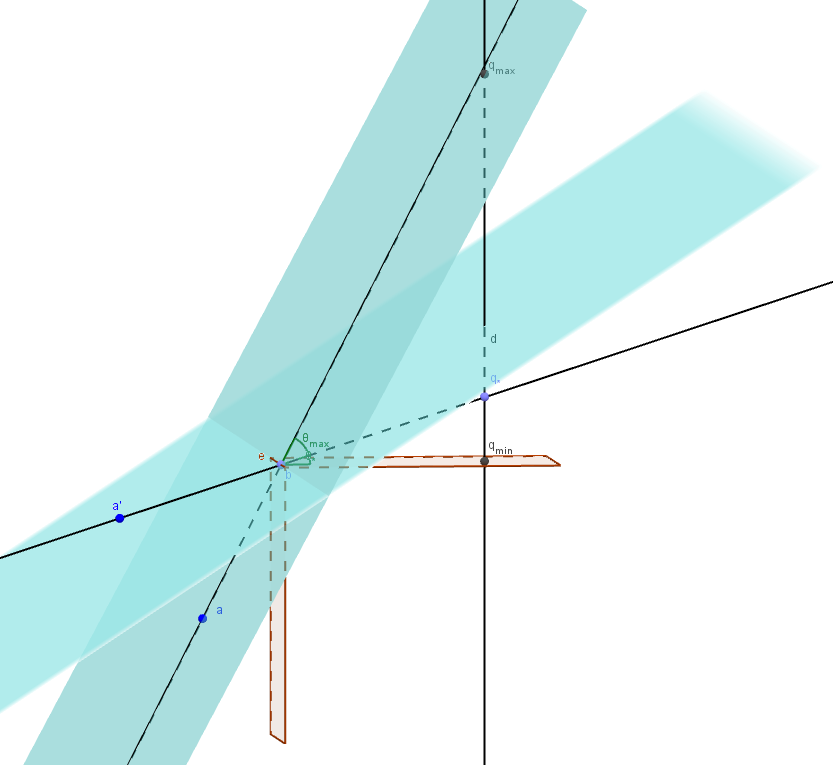
\includegraphics[scale=0.9]{path3D.png}
\caption{Scene}
\end{figure}


\end{document}
